\section{Example: The API and Structure of LMFDB}\label{sec:sota}

The ``L-functions and Modular Forms Database'' (\lmfdb~\cite{lmfdb}) is a Python web
application with a MongoDB backend.  The project contains several thousand L-Functions and
curves along with their properties. We use this as an example of a Virtual Theory.  Before
we go into this in more detail, we first have a closer look at the structure and existing
APIs to communicate with it.

\subsection{The Structure of LMFDB}\label{sec:sota:struct}

\lmfdb has several sub-databases -- each of which contains different kinds of objects.
These databases include e.g. a database of elliptic curves or a database of transitive
groups.  Within each database, each curve is stored as a single JSON record with common
keys, Figure~\ref{fig:lmfdbexample} shows one: each property of this JSON object corresponds to a property of the underlying mathematical object. 
For example, the \identifier{degree} property -- here $1$ -- of the JSON objects corresponds to the degree of the underlying elliptic curve. 


\begin{figure}[ht]\centering
      \begin{lstlisting}[language=json]
{
    "degree": 1,
    "non-maximal_primes": [5],
    "torsion_structure": ["5"],
    "ainvs": ["0","-1","1","-10","-20"],
    "x-coordinates_of_integral_points": "[5,16]",
    "real_period": 1.26920930427955,
    "min_quad_twist": {"disc": 1,"label": "11a1"},
    "sha_an": 1.0,
    "conductor": 11,
    "iwp0": 7,
    "2adic_gens": [],
    "torsion_primes": [5],
    "signD": -1,
    "tamagawa_product": 5,
    "isogeny_matrix": [[1,5,25],[5,1,5],[25,5,1]],
    "non-surjective_primes": [5],
    "lmfdb_label": "11.a2",
    "2adic_index": 1,
    "equation": "\\( y^2 + y = x^{3} -  x^{2} - 10 x - 20  \\)",
    "label": "11a1",
    "regulator": 1.0,
    "anlist": [0,1,-2,-1,2,1,2,-2,0,-2,-2,1,-2,4,4,-1,-4,-2,4,0,2],
    "iso": "11a",
    "_id": "ObjectId('4f71d4304d47869291435e6e')"
}
      \end{lstlisting}\vspace*{-1.5em}
  \caption[An elliptic curve from \lmfdb]{
    An elliptic curve, as found within \lmfdb. 
    Some key-value pairs are omitted for readability. 
  }
  \label{fig:lmfdbexample}
\end{figure}

Other properties are more complex.
Whereas the value of the \identifier{degree} property is a simple integer, the value of
the \identifier{isogeny\_matrix} property is a list of lists, which represents a matrix. 
This can become even more technical. 
For example the \identifier{x-coordinates\_of\_integral\_points} field, \lmfdb represents
a list of integers as a list of strings as the integers can exceed the range of MongoDB system
integers.  This already shows that it is non-trivial to get from a MongoDB encoding of an elliptic
curve in \lmfdb to the representation of a mathematical object. 


\subsection{An API for \lmfdb Objects}\label{sec:sota:api}

As \lmfdb is is a mathematical knowledge base, one important use case is to find elliptic
curves subject to specific criteria. As a very simple example, suppose a mathematician
wants to find all Abelian elliptic curves.  How can this be achieved using the \lmfdb API
at \url{http://www.lmfdb.org/api/}\ednote{Proper citation}.

\begin{figure}[ht]\centering
  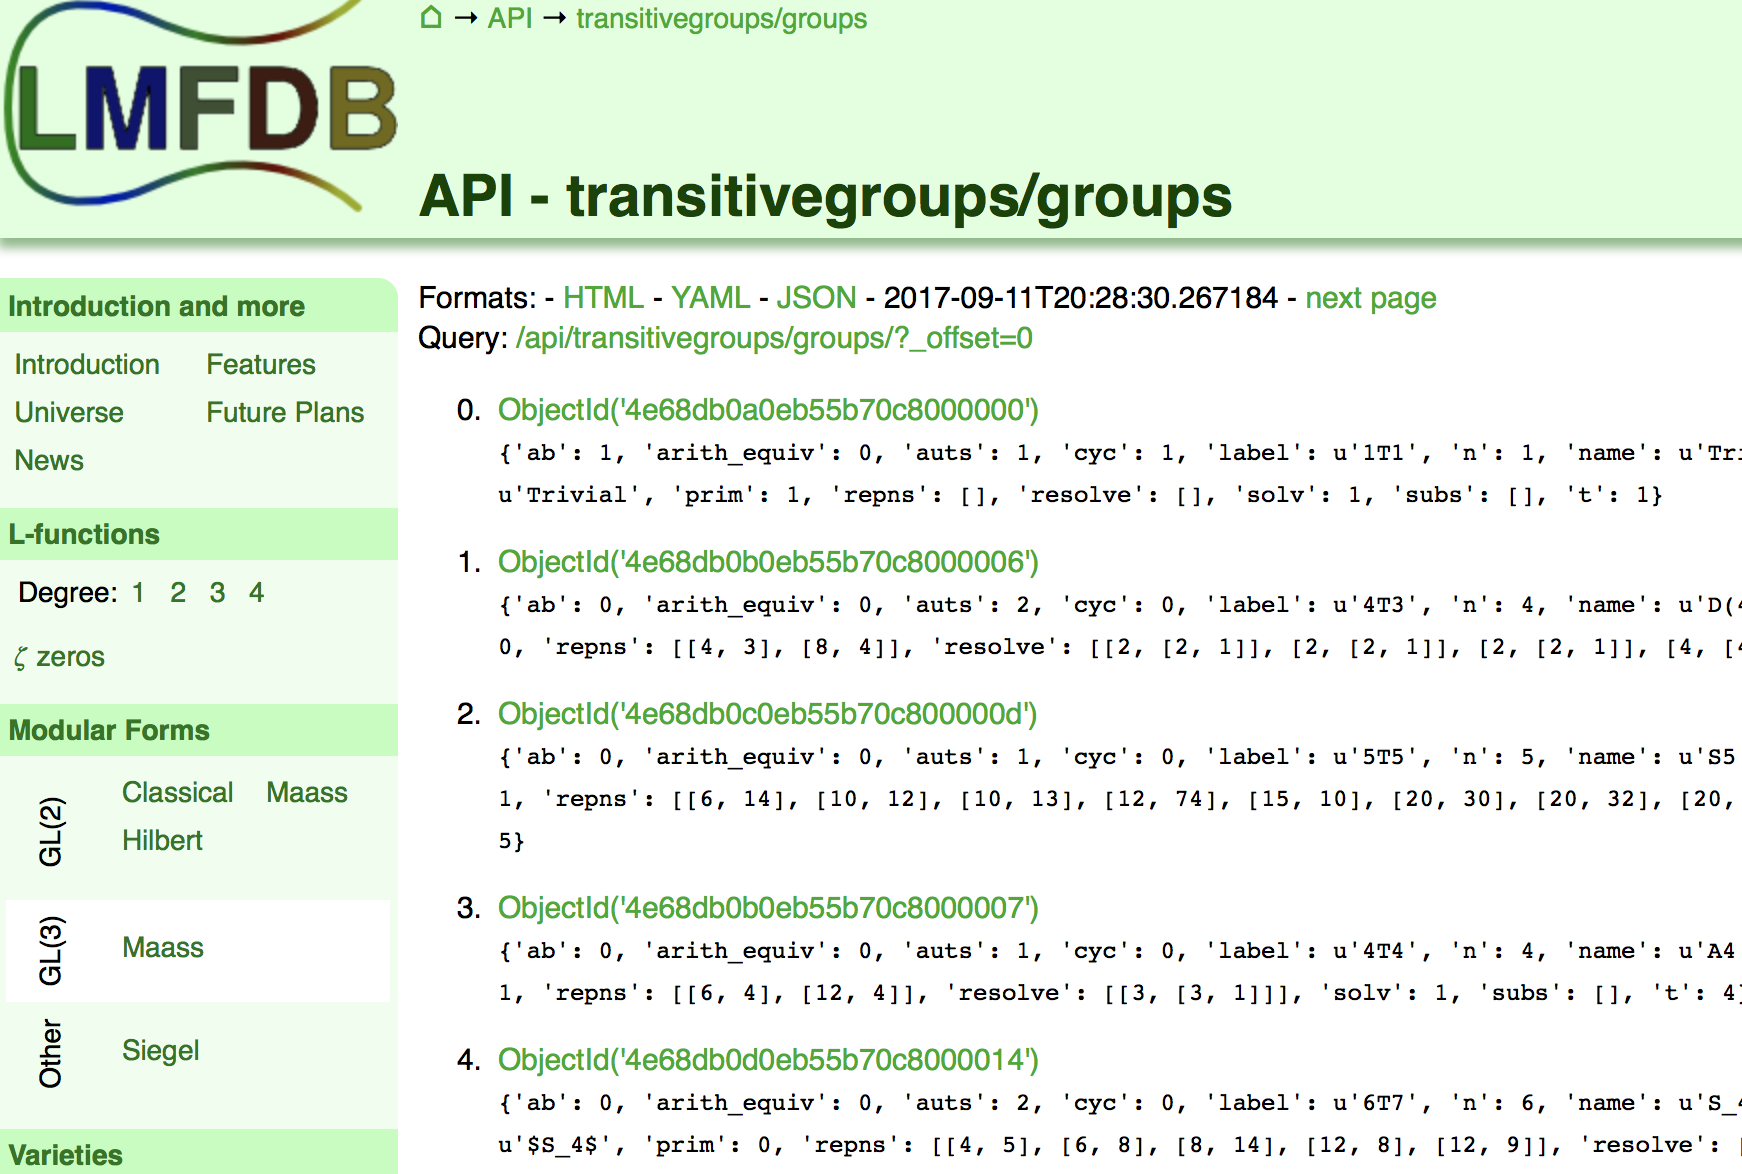
\includegraphics[width=\textwidth]{APIScreenshot.png}
  \caption[The Web-Interface for the \lmfdb API. ]{
    The Web-Interface for the \lmfdb API. 
  }
  \label{fig:apiscreenshot}
\end{figure}

This API has two basic modes. The first allows allows to make searches using the
web-browser.  Users can manually enter a query, and see a list of results displayed.  A
screenshot of this interface is shown in Figure~\ref{fig:apiscreenshot}.  In the other
mode queries can be given as JSON directly.  This can be used in automated scenarios.

In both of these mods queries must be formulated in terms of the underlying MongoDB
schema. For example, to search for all abelian elliptic curves, we must know that the
\identifier{ab} key corresponds to the commutativity property, has Boolean values, and
that MongoDB encodes \inlinecode{true} as \inlinecode{1}, and \inlinecode{false} as
\inlinecode{0} in this \lmfdb sub-database. This information can then be used to make a
request to \url{http://www.lmfdb.org/api/transitivegroups/groups/?ab=1}. This finds all
Abelian, transitive groups.

In this example, each of the steps are relatively straightforward. 
In a general setting, e.g. when searching for all elliptic curves with a specific isogeny
matrix, this not only requires a good familiarity with the mathematical background but
also with the system internals of the particular \lmfdb sub-database; a skillset commonly
found in neither research programmers nor average mathematicians.   

To summarize: while \lmfdb offers a programmable API for accessing its contents, the
content API is at the MongoDB level, and not the level of mathematical objects. Our
Diagnosis is that \lmfdb -- and most other mathematical knowledge databases -- suffer from
a double impedance mismatch problem.
\begin{compactenum}[\bf {I}1]
\item \emph{human/computer impedance mismatch}: Humans have problems interacting with
  \lmfdb, since they must speak the system language instead \lmfdb speaking mathematics
\item \emph{computer/computer impedance mismatch}: mathematical computer systems cannot
  interoperate, since their system languages differ.
\end{compactenum}
In the MitM approach we have presented in Section~\ref{sec:mmtmitm}, we can solve both
problems at the same time by lifting the communication to the level of \ommt-encoded MitM
objects, which both MitM-compatible software systems and humans speak -- this is the
central assumption of the MitM approach.
%%% Local Variables:
%%% mode: latex
%%% TeX-master: "paper"
%%% End:

%  LocalWords:  sec:sota lmfdb lmfdb lstlisting json ainvs iwp0 2adic_gens isogeny_matrix
%  LocalWords:  tamagawa_product 2adic_index anlist 4f71d4304d47869291435e6e vspace emph
%  LocalWords:  fig:lmfdbexample isogeny includegraphics textwidth fig:apiscreenshot
%  LocalWords:  centering summarize sec:mmtmitm ommt-encoded
